\documentclass[jou]{apa6} %draft apacite

\usepackage[style=authoryear,sorting=nyt,backend=bibtex]{biblatex}
\usepackage{csquotes}
\usepackage{hyperref}
\usepackage{soul}
\usepackage{graphicx}
\graphicspath{ {figures/} }

\addbibresource{lit.bib}

\title{ASRAEL - Acquisition of Semantic RelAtions bEtween Latin nouns}
\shorttitle{APA style}

\author{Konstantin Schulz}
\affiliation{Humboldt-Universität zu Berlin}

\abstract{XXXabstractXXX}

\rightheader{ASRAEL}
\leftheader{Konstantin Schulz}

\begin{document}
\maketitle    
\tableofcontents
\listoffigures
\listoftables
                        
\section{Introduction}

This dissertation deals with different ways of detecting semantic relations in text corpora. Its focus is more on methodology than on analytical results. Some important restrictions are necessitated by the precise research question: In a corpus of Latin texts, how can we automatically extract semantic relations that are relevant for language learning? I will concentrate only on a subset of the existing phenomena, namely hypernymy and hyponymy. This selection is motivated by the objective of utilizing the obtained insights as the basis for exercises in the process of learning historical languages. Thus, the detection of said relations is not an end in itself, but is to be viewed in the context of how humans learn languages. 

\subsection{Semantic relations in language learning}

Specifically, recent studies suggest that an improved integration of hyponymy into the learning process can lead to a higher level of language skills: 
\blockquote[{\cite[p.~196]{taslimExperimentalStudyTeaching2014}}]{[...] Hyponymy games are highly effective in developing students' level of vocabulary [...].}
Roughly the same procedure is applicable also in the context of artificial intelligence, which highlights the general importance of semantic relations in any kind of language learning effort:
\blockquote[{\cite[p.~1306]{carlsonArchitectureNeverendingLanguage2010}}]{At present, [Never-Ending Language Learner] acquires two types of knowledge: (1) knowledge about which noun phrases refer to which specified semantic categories, such as cities, companies, and sports teams, and (2) knowledge about which pairs of noun phrases satisfy which specified semantic relations, such as hasOfficesIn(organization, location).}
The automated extraction of semantic relations from texts can be used for constructing ontologies in specific domains, which is important for language learning because many textbooks are heavily structured according to a range different topics:
\blockquote[{\cite[p.~192f.]{punuruLearningNontaxonomicalSemantic2012}}]{[Ontologies] allow machines to comprehend the semantics of documents and return more accurate answers to user queries. As of now, ontologies for domains of interests are developed manually in spite of the wide spread use of ontologies. This situation clearly indicates the urgent need for techniques that can automatically learn (construct) ontology from domain texts.}
Since there is a parallel between semantic relations (or ontologies in general) and the way that humans think, it seems reasonable to exploit that connection for learning purposes. This is particularly important for advanced learners' lexical acquisition:
\blockquote[{\cite[p.~56]{crossleyDevelopmentSemanticRelations2010}}]{While it may be true that explicit vocabulary instruction concentrating on the first 2,000 to 3,000 words is valuable for the beginning learner [...], it is generally agreed that subsequent vocabulary acquisition results from inference strategies and the development of word connections [...].}
Now, one might be tempted to conclude that predefined lists of basic vocabulary and more advanced semantic relations would be a sufficient help to language teachers. However, static materials und human supervision will probably fail to account for the entire processual complexity of lexical acquisition:
\blockquote[{\cite[p.~71]{crossleyDevelopmentSemanticRelations2010}}]{[...] since lexical acquisition is a phenomenon that is generally too complex to be analyzed based on human intuition, computational approaches are beneficial.}
The involvement of artificial intelligence in the modeling of human knowledge about vocabulary faces various problems, including the progression of learning over time:
\blockquote[{\cite[p.~70]{crossleyDevelopmentSemanticRelations2010}}]{[...] L2 learners begin to develop closer semantic similarities between speech segments as they progress in acquiring a second language.}
In language learning contexts, this problem extends also to the morphological domain, where it can prove difficult for students to exploit their knowledge about affixation for the acquisition of semantic relations:
\blockquote[{\cite[p.~248]{gardnerValidatingConstructWord2007}}]{Extant research in this regard suggests that [initial and extensive exposure to a stem through inflected and derived forms, rather than base forms,] may be more difficult for learners.}
However, "inflected and derived forms" are exactly what we encounter in the curricular targets for Latin courses, i.e. literary texts. Most textbooks take care of the problem by using hand-crafted Latin texts instead of authentic ones. This leads to a highly problematic transition from textbook to literature, which is already famous among German teachers of Latin:
\blockquote[{\cite[p.~115]{schibelZurAneignungLateinischer2013}}]{Die Antwort gibt die von Lateinlehrern oft zu hörende Klage über einen ,Lektüreschock‘, den Schüler beim Übergang vom Lehrbuch zu Originaltexten erleiden. Die wohlmeinende Sorge der Verfasser lateinischer Lehrwerke für einen allmählichen, von Lektion zu Lektion sparsam dosierten Anstieg der sprachlichen Anforderungen zeitigt einen langen Aufenthalt der Lerner in einer fabrizierten Sprachwelt, die nicht zur Überwindung sprachlicher Hürden anspornt.}
The challenge, then, is to not only extract semantic relations from a given corpus, but also to group them according to general principles of progression that are tightly coupled with a domain-specific theory of learning.

\subsection{Word Sense Induction}
\label{polysemyProblemForSemanticRelations}

In order to reach that point, we first need to define the basic object to be acquired, i.e. semantic relations. Unfortunately, this is not a precisely defined research object per se because it strongly depends on our previous knowledge about the possible word senses:
\blockquote[{\cite[p.~12]{ayseExtractionSemanticWord2011}}]{For more accurate semantic analysis, the connection between words should be established between appropriate senses of the words. To be more concrete, an example can be given on the semantically ambiguous word as; yüz ‘face’ or ‘hundred’. When a has-a relation is detected between the words vücut ‘body’ and yüz, the appropriate sense for yüz should be selected as ‘face’, instead of ‘hundred’.}
Consequently, the sense of a word has to be defined before we can start to learn more abstract representations like hyponymy:
\blockquote[{\cite[p.~137]{bartunovBreakingSticksAmbiguities2016}}]{[...] the problem of learning multi-prototype word representation is closely related to word-sense induction [...].}
Further obstacles may occur in the case of specific relations like synonymy, where a good operationalization is needed to retrieve the relevant instances from a corpus of text data:
\blockquote[{\cite[p.~274]{divjakCorpusbasedCognitiveSemantics2009}}]{Polysemy requires the researcher to determine whether two usage events are identical or sufficiently similar to be considered a single sense, what the degree of similarity is between different senses, where to connect a sense to others in the network, and which sense(s) to recognize as prototypical one(s). [...] in addition, [linguists] have to decide what the differences are between the near-synonyms as well as what the relation is between semantically similar words in a domain.}
In my study, I will focus heavily on the approach of distributional semantics, describing specific semantic relations between words in terms of their co-occurrences, i.e. typical contexts in a corpus. This approach has traditionally suffered from several limitations. In some cases (e.g. synonymy), building unified vectors for every type in a corpus can prove highly problematic:
\blockquote[{\cite[p.~114]{karanDistributionalSemanticsApproach2012}}]{Distributional representations of each sense of a polysemous word get merged into a single distributional representation – a mixture of distributions. For questions with high polysemy level, the corresponding distributional vectors are blurred and the similarity comparisons between such vectors are less meaningful.}
However, this is not universally true anymore as there are models that consistently distinguish between various contexts (\hyperlink{ELMO}{see below}). Other problems of distributional semantics are tied to fine-grained distinctions between specific semantic relations:
\blockquote[{\cite[p.~115]{karanDistributionalSemanticsApproach2012}}]{However, manual inspection revealed that most false synonyms are syntagmatically related to the target word. To avoid this kind of error, we would need a method to distinguish between synonymy and general semantic relatedness.}
Plain co-occurrence counts can be a good basis for the detection of semantic relations in general, but they are rarely sufficient for a thorough classification into several subcategories. Nonetheless, previous research has been carried out (more or less successfully) using, e.g., association measures to detect synonymy:
\blockquote[{\cite[p.~566]{hagiwaraSupervisedSynonymAcquisition2009}}]{The value of distributional features \( f_j^D (x, z) \) is determined so that it represents the degree of commonality of context \( c_j \) shared by the word pair (x, z). [...] The advantage of this feature construction is that, given the independence assumption between word x and z , the feature value is easily calculated as the simple sum of two corresponding pointwise mutual information weights as: \( f_j^D (x, z) = PMI(x, c_j) + PMI(z, c_j) \) [...].}
One of the critical parts in that view is the term "word pair", which introduces the linguistically ill-defined concept of word into an otherwise seemingly precise mathematical formula. In the following, we will start by using the term "word" simply as a synonym of "token" and later proceed to a more advanced definition. This progression seems reasonable given the fact that the usage of bare token-based PMI (Pointwise Mutual Information) for distributional questions may lead to severely skewed results:
\blockquote[{\cite[p.~444]{herbelotMeasuringSemanticContent2013}}]{[...] strong collocation effects can influence the measurement of information negatively: it is an open question which phrases should be considered ‘words-with-spaces’ when building distributions.}
Therefore, corpora may have to be tokenized and segmented using more complex separator rules than "whitespace and punctuation" before they can serve as a basis for distributional analyses. Besides, polysemy itself may also become a problem for resolving other issues like synonymy, e.g. if two words are synonymous only in one of their possibly numerous senses:
\blockquote[{\cite[p.~444]{herbelotMeasuringSemanticContent2013}}]{Some of the errors we observe may also be related to word senses. For instance, the word medium, to be found in the pair magazine – medium, can be synonymous with middle, clairvoyant or again mode of communication. In the sense of clairvoyant, it is clearly more specific than in the sense intended in the test pair. As distributions do not distinguish between senses, this will have an effect on our results.}
In addition to polysemy itself, related concepts like homonymy can also become obstacles with regard to the aim of precisely defining semantic relations:
\blockquote[{\cite[p.~251]{gardnerValidatingConstructWord2007}}]{This potential for meaning variation (both homonymy and polysemy) becomes even more convoluted when the morphological word family is considered. For instance, forms that appear to be related through affixation may actually be homographs in context (e.g. bear, the animal, and bears/bearing, the verb meaning to carry) [...].}
Distributional semantics provides a valuable framework to break down the multiple aspects of meaning for homonymous or polysemous words into smaller subsets, based on the combination with, e.g., adjectival modifiers:
\blockquote[{\cite[p.~42]{boledaIntensionalityWasOnly2013}}]{It is plausible that modifying a noun has a larger impact when the noun is polysemous, as the adjective narrows down the meaning of the noun; indeed, adjectives have been independently shown to be powerful word sense disambiguators of nouns [...]. In distributional terms, the adjective notably “shifts” the vector of polysemous nouns, but for monosemous nouns there is just not much shifting room.}
Therefore, the integration of specific contextual elements into the analysis of hyponymy between Latin nouns seems to be a reasonable basis for distinguishing subtle semantic nuances more consistently. As a consequence, polysemy will be treated in this study not just as one of the analytical targets, but also as a methodological aspect that needs to be addressed before other kinds of analyses can be performed. A useful operationalization of polysemy in a distributional context could be to look at the collocational diversity:
\blockquote[{\cite[p.~8]{hamiltonDiachronicWordEmbeddings2016}}]{We construct empirical co-occurrence networks for the top-10,000 non-stop words of each language using the PPMI measure [...]. In these networks words are connected to each other if they co-occur more than one would expect by chance (after smoothing). The polysemy of a word is then measured as its local clustering coefficient within this network [...].}
This approach brings along the problem of sampling, which is a general one for the whole of corpus linguistics: If we want to model a specific language like Latin as a whole but only use a tiny subset of the available language data for our corpus, how can we expect our results to be reliable, i.e. reproducible in similar research environments? The key point here is the purpose: For this study, our ultimate goal is not to model Latin nouns per se, but only with regard to the rather well-defined application context of language learning. Therefore, the explanatory power of our linguistic model can be much smaller because it will be restricted to predefined parameters. These parameters may in turn be described as, e.g., the objective of maximizing a student's learning success by providing structured information about semantic relations.

\subsection{Hyponymy}

After dealing with various issues of polysemy, some of the second-tier relations may have to be redefined when looked at from a distributional perspective, e.g. hyponymy:
\blockquote[{\cite[p.~443]{herbelotMeasuringSemanticContent2013}}]{Although \textit{beverage} is an umbrella word for many various types of drinks, speakers of English use it in very particular contexts. So, distributionally, it is not a ‘general word’.}
In this view, other existing taxonomies that may have acted as models of hyponymy need to be replaced by a definition that reflects how actual usage contexts can limit our selection of possible candidates for hyponymy:
\blockquote[{\cite[p.~443]{rollerInclusiveSelectiveSupervised2014}}]{[The Distributional Inclusion Hypothesis] states that more specific terms appear in a subset of the distributional contexts in which more general terms appear. So, \textit{animal} can occur in all the contexts in which \textit{dog} can occur, plus some contexts in which dog cannot – for instance, rights can be a typical cooccurrence for animal (e.g. “animal rights”), but not so much for dog (e.g. \#“dog rights”).}
Unfortunately, this view may clash with the observations of \cite{herbelotMeasuringSemanticContent2013}:
\begin{itemize}
      \item Hypernyms can have very specific usage contexts.
      \item Collocations may lead to unexpected results in the distribution of words.
\end{itemize}
Similar adjustments have to be made in treating other kinds of semantic relations. Therefore, many researchers apply preprocessing to their corpora before performing the actual analysis on them:
\blockquote[{\cite[p.~56f.]{gyllenstenRgramsUnsupervisedLearning2019}}]{It is worth noting that the skipgram model uses subsampling of common words, which is an optimization introduced to compensate for the power law distribution in common vocabularies. Also, the skipgram model controls for collocations by dampening the impact of frequent collocations.}
However, this increases the danger of circularity, revealing only those results that we were already expecting in the first place. As an alternative, we should look for a model that is robust enough to detect semantic relations despite the confounding factors. The objective should be to fit the model to the base text, not the other way round. For creating word embeddings using the skipgram model, subsampling and the restriction of strong collocations may be justified from a computational perspective because they enable a faster training of models while more or less preserving the resulting performance in the prediction of word contexts. This very tradeoff, though, may not work out as well for the detection of semantic relations, e.g. if we give a higher priority to the frequency of certain contexts. Such a change of algorithm may particularly be motivated by the distinction of theoretical and empirical scopes of words:
\blockquote[{\cite[p.~46]{coenenAnalogieUndMetapher2013}}]{Theoretischer Anwendungsbereich eines Wortes: die Klasse der Gegenstände, auf die ein Wort kraft seiner Bedeutung beschreibend angewandt werden kann (TA). Empirischer Anwendungsbereich eines Wortes: die Menge der Gegenstände, zu deren Beschreibung ein Wort - bis zu einem gewissen Zeitpunkt - in der Erfahrung eines bestimmten SprachteiInehmers bereits angewandt wurde (EA).}
This may be transferred to the domains of corpus linguistics and language learning: Given a text corpus that includes a learner's desired knowledge (e.g. all the literature one wants to read), the theoretical scope of a certain word would be equivalent to all the distinct relevant contexts in the corpus in which that word occurs. In contrast, the empirical scope of that same word would be equal to the number of distinct relevant contexts in the corpus in which it occurs \hl{and} which are known to the learner (at any given point in time of his learning process). Thus, the theoretical scope will remain static as long as we do not change the corpus, while the empirical one will always be dynamic in any case. From this point of view, we can also restrict our notion of semantic relations: Hyponymy, for instance, will be tied to those word networks that are present in a specific corpus and, for a learner, specific instances of hyponomy relations will not exist unless they have already been part of a learning situation. It is therefore our duty to a) detect such instances in the corpus and b) use them to design learning situations that help language learners to build lexical knowledge. In order to accomplish that first part, we need to have clearly defined requirements to qualify a relation as one of hyponymy:
\blockquote[{\cite[p.~16]{gevaudanSemantischeRelationenNominalen1999}}]{Auf der konzeptuellen Ebene, auf der auch Similarität und Kontiguität angesiedelt sind, beruht Hyponymie auf der taxonomischen Inklusion von Konzepten. Die taxonomische Inklusion ist nichts anderes als eine Ober-/Unterbegriffsbeziehung [...]. Diese Konzeptpaare sind teilidentisch, weil die Extension (die Menge der mit dem Begriff gemeinten Phänomene) des Unterbegriffs in der des Oberbegriffs enthalten ist und gleichzeitig die Intension (die Menge der dem Begriff zugeordneten Eigenschaften) des Oberbegriffs in der des Unterbegriffs enthalten ist [...].}
This notion of semantic super- and subordination between words closely resembles the general principles in cognitive linguistics (\cite[p.~5]{nerlichPolysemyFlexibilityIntroduction2003}).
\begin{figure}[ht]
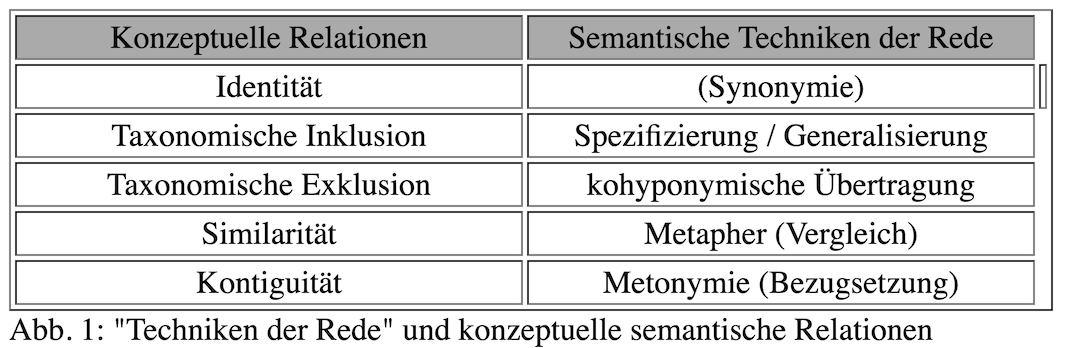
\includegraphics[width=\linewidth]{hyponymy_generalization_specification}
\caption{Hyponymy as generalisation/specification (\cite[p.~18]{gevaudanSemantischeRelationenNominalen1999})}
\label{figure:hyponymyAsGeneralisation}
\end{figure}
If hyponymy refers to some underlying taxonomy in which a hyponym is subordinate to its hypernym (see Figure ~\ref{figure:hyponymyAsGeneralisation}), our most important task will be to establish that taxonomy in a corpus-based manner. Therefore, lexical resources like the Latin WordNet (\cite{minozziLatinWordNetProject2010}) may contribute a reference model for such a purpose because it includes a built-in notion of hyponymy. Unfortunately, the WordNet defines such relations based on intuition, not on actual language use:
\blockquote[{\cite[p.~315]{fellbaumChallengesMultilingualWordnet2012}}]{WordNet’s original motivation was to test the feasibility of a model of human semantic memory that sought to explain principles of storage and retrieval of words and concepts.}
WordNet is therefore static and non-empirical from the perspective of usage-based fields like corpus linguistics. However, since it was supposedly constructed by experts, we may use their assessment for evaluating the corpus-based extraction of hyponymy. This kind of approach is supported by recent studies:
\blockquote[{\cite[p.~984-988]{onoWordEmbeddingbasedAntonym2015}}]{The WE-T model receives supervised information from synonym and antonym pairs in thesauri and infers the relations of the other word pairs in the thesauri from the supervised information. The WE-TD model incorporates corpus-based contextual information (distributional information) into the WE-T model, which enables the calculation of the similarities among in-vocabulary and out-of-vocabulary words. [...] Our WE-TD model achieved the highest score among the models that use both thesauri and distributional information.}
According to \cite{onoWordEmbeddingbasedAntonym2015}, it is not sufficient to use thesauri like the WordNet for detecting semantic relations; rather, we should use that as a basis and provide additional information from actual corpora, thereby combining the taxonomic (i.e. introspective) and the distributional (i.e. usage-based) approach to semantics. The former can be helpful in two ways: a) by defining a horizon of expectations in language learning contexts, i.e. which information learners are supposed to infer from their previous knowledge in order to understand a linguistic expression in a specific text passage; and b) by modeling semantic knowledge in a machine-readable, consistent (albeit simplistic) manner. The integration of distributional semantics, on the other hand, is particularly motivated by the hypothesis that semantic properties of words are reflected in their contextual surroundings:
\blockquote[{\cite[p.~59]{griesBehavioralProfilesCorpusbased2009}}]{[...] distributional similarity reflects, or is indicative of, functional similarity, the understanding of functional similarity being rather broad, i.e. encompassing semantic, discourse-pragmatic, and other functions a particular expression can take on.}
Using distributional corpus data, we also gain the advantages of rigorously empirical research (as opposed to bare intuition and anecdotal evidence): frequency, authenticity, variation and systematic induction.
\blockquote[{\cite[p.~60]{griesBehavioralProfilesCorpusbased2009}}]{[In contrast to introspection,] corpora a. provide many instances rather than a few isolated judgments; b. provide data from natural settings rather than 'armchair' judgments or responses that potentially reflect experimentally-induced biases; c. provide co-occurrence data of many different kinds, i.e. not just those a particular researcher may consider important; d. and thus, allow for bottom-up identification of relevant distinctions as well as for a more comprehensive description than is typically provided.}
Still, taxonomic knowledge may be useful for languages like Latin where previous research is scarce and, more often than not, heavily introspective or anecdotal. In both the taxonomic and the distributional case, we can increase the amount of provided information by relying on associated properties of hyponymy relations, e.g. transitivity:
\blockquote[{\cite[p.~58]{coenenAnalogieUndMetapher2013}}]{Die Relationen der Hyper- und Hyponymie sind transitiv. Wenn A Hyponym in Bezug auf B ist, dann auch in Bezug auf die Hyperonyme von B, und wenn B Hyperonym in Bezug auf A ist, dann auch in Bezug auf die Hyponyme von A.}
Applied to the Latin WordNet, this may look as follows:
\begin{enumerate}
         \item \textit{gladius}
         \item a cutting or thrusting weapon with a long blade
         \item weaponry used in fighting or hunting
         \item weapons considered collectively
         \item an artifact (or system of artifacts) that is instrumental in accomplishing some end
         \item a man-made object
         \item a physical (tangible and visible) entity
\end{enumerate}
This information flow can be read from both sides. Beginning at \textit{gladius} (sword), it can be used to simulate the process of reading a text: We encounter a word in the text (e.g. the plural \textit{gladii}) and determine its lemma (\textit{gladius}). From there, we can try to find a corresponding meaning for the surface form, e.g. "a cutting or thrusting weapon with a long blade". This meaning, in the WordNet taxonomy, can be hyponym to other kinds of meaning, e.g. "weaponry used in fighting or hunting". Now, if we know that
\begin{itemize}
         \item \textit{gladius} is a weapon with a blade and
         \item weapons with a blade can be used for hunting,
\end{itemize}
then we are safe to assume that a \textit{gladius} can be used for hunting. The further we go down the list, the more abstract do the meanings get. Nonetheless (or because of that), every layer can remind us of new specific features that we may want to associate with \textit{gladius}: specific motion (2.), specific purpose (3.), hypernym (4.), general purpose (5.), origin and production (6.), material (7.). In some cases, we may even use morphological hints to get faster access to information about hyponymy:
\blockquote[{\cite[p.~913]{anstattTypenSemantischerRelationen2009}}]{[...] zur Bildung von Hyponymen kann z.B. das Suffix -ovye/-evye (seld’ ‚Hering‘ – sel’devye ‚Heringsartige‘) verwendet werden (s. Ginzburg 1985, 9).}
This is especially true for Latin with its relatively rich morphology: the meaning of \textit{artifex} (artist) may be associated directly to \textit{ars} (art) and \textit{facere} (to make), without necessarily traversing a hierarchical chain of increasing generalisation. Interestingly, this is possible even in cases where the compound is formed from foreign language material and thus cannot be easily paraphrased in the native language:
\blockquote[{\cite[p.~33]{souille-rigautSemanticAccountQuasiLexemes2010}}]{The head constituent in both compounds is on the right, the modifier constituent on the left, and, although ‘cardiopathy’ is not paraphrasable, we can still deduce from its semiotic units that the compound as a whole is a hyponym of the meaning carried by the semiotic unit -path-.}
How is that important for Latin hyponymy? Consider Greek loanwords, e.g. \textit{xylophytum} (a certain kind of plant) cannot be described in Latin words as a \textit{*phytum} that is made of \textit{*xylum}. However, Romans may have deduced that the meaning of \textit{xylophytum} is related to ($\rightarrow$ hyponymy) \textit{-phyt-}, thereby inferring previous knowledge about plants. Therefore, we have to allow for the possibility that some instances of hyponymy may not be extractable solely on a distributional basis, but rather on a morphological one. Besides, a morphologically informed model is able to explain why we can immediately see semantic structure in newly coined words:
\blockquote[{\cite[p.~43]{souille-rigautSemanticAccountQuasiLexemes2010}}]{‘Dontopedalogy is the science of opening your mouth and putting your foot in it, a science which I have practiced for a good many years’. There is evidence that we are dealing with a secondary compound of the type W + X + Y, that is to say, with the semiotic units -dont- + -ped- + -log- being concatenated synchronically. [...] secondary compounds W + XY are always expanded primary compounds in which WXY is a hyponym of XY.}
In this respect, knowledge about specific hyponyms or hyponymy in general can facilitate the language learning process by providing a rather intuitive access to the meaning of single words or phrases. Unfortunately, this intuition sometimes competes with other interpretations of a word's sense which may be equally intuitive and valid:
\blockquote[{\cite[p.~126]{ponsborderiaPathsGrammaticalizationSpanish2014}}]{(29) Y en ese convento nos regalaron diversas veces con tortillas de huevos [...]. Un día, o sea una tarde, salimos de dicho convento de San Diego, adonde habíamos merendado muy bien de dichas tortillas (1705, Raimundo de Lantery, Memorias)
'In that convent we were given egg omelettes several times [...] One day, or be-SBJV one afternoon, we went out of this convent of San Diego, where we had a tasty snack of such omelettes'
In (29), o sea links two words, which can be interpreted as either hyperonym > hyponym (day > afternoon), or exclusive co-hyponyms (morning V afternoon).}
Such examples underline the importance of disambiguation (\hyperref[polysemyProblemForSemanticRelations]{see above}), which may not always be possible. Furthermore, additional steps may be necessary even if a specific word sense was already determined, e.g. the inference of common knowledge or common sense:
\blockquote[{\cite[p.~427f.]{pinkalSemantik1993}}]{[...] die Semantikkonstruktion [...], die das semantische Potential auf der Grundlage der lexikalischen und syntaktischen Information ermittelt, die in der Eingabekette enthalten ist; [...] die semantische Resolution, die den aktuellen semantischen Wert bestimmt, unter anderem durch die Auflösung von Mehrdeutigkeiten (Disambiguierung) und [...] die semantische Auswertung, die durch die Anwendung von Deduktions- und Inferenzmechanismen auf den semantischen Wert einer Äußerung die relevante Äußerungsinformation extrahiert und dabei unter anderem Weltwissen (episodisches Wissen und Regelwissen) einbezieht.}
In this view, disambiguation should be preceded by a thorough linguistic analysis of the context, which, in terms of distributional semantics, is usually addressed by extracting cooccurrence frequencies from sliding windows over a textual input, be it plain text or a linguistically annotated treebank. However, the integration of external information into this process is not as straightforward and therefore often avoided. In the end, this might not be the worst decision, depending on our definition of semantics: Some models of distributional semantics reduce the spectrum of polysemy to one main aspect of meaning per word.
\blockquote[{\cite[p.~4]{faruquiProblemsEvaluationWord2016}}]{However in [the dataset] WS-353, bank is given a similarity score of 8.5/10 to money, signifying that bank is a financial institution. Such an assumption of one sense per word is prevalent in many of the existing word similarity tasks, and it can incorrectly penalize a word vector model for capturing a specific sense of the word absent in the word similarity task.}
\hypertarget{ELMO}{Approaches} of this kind level nuances that may be actually important for our understanding of a single word in its context. As an improvement, other models regard entire sentences for the representation of a word's context-specific meaning, thereby differentiating between various common usages: 
\blockquote[{\cite[p.~2f.]{petersDeepContextualizedWord2018}}]{Given a sequence of N tokens, (t1, t2, ..., tN), a forward language model computes the probability of the sequence by modeling the probability of token tk given the history (t1, ..., tk-1) [...]. A backward LM is similar to a forward LM, except it runs over the sequence in reverse, predicting the previous token given the future context [...]. A biLM combines both a forward and backward LM. Our formulation jointly maximizes the log likelihood of the forward and backward directions [...].}
Modeling the process of language production both in a forward and backward manner at the same time seems reasonable, especially for the Latin language, because the antecedent of, e.g., a relative pronoun can become part of the relative clause, which makes it difficult to understand the structure of such a construction by reading it in just one direction, without referring to the past and future context at the same time:
\blockquote[{PROIEL 53467}]{Nam et frumentum ex agris cotidie in castra conferebat et quae gravissime adflictae erant naves earum materia atque aere ad reliquas reficiendas utebatur [...].}\footnote{For details on the PROIEL corpus, see \cite{haugCreatingParallelTreebank2008}. Note that in this study, for the PROIEL corpus, unique sentence identifiers will be used to refer to text passages of ancient works. This is often more precise than the conventional citation model (in this case: Caes. BG 4.31.2) and does not require knowledge about abbreviations of author names or work titles. On the downside, it is corpus-specific and does not offer immediate information about author, work and structural position of the passage.}
In this example, \textit{naves} is the antecedent to the relative pronoun \textit{quae}. Its integration into the relative clause is recognizable by its case congruency with the relative pronoun. In a more conventional setting, the sentence would look like this: \textit{[...] conferebat et earum navium, quae gravissime adflictae erant, materia atque [...]}. Such syntactic variations are probably related to the relatively free word order in the Latin language. Therefore, a language model for Latin should be flexible enough to analyze a given textual sequence by looking at either the left or right context, according to the circumstances of the case:
\blockquote[{\cite[p.~8]{devlinBertPretrainingDeep2018}}]{(b) [Concatenating separate Left-To-Right and Right-To-Left models] is non-intuitive for tasks like [Question Answering], since the [Right-To-Left] model would not be able to condition the answer on the question; (c) [this] is strictly less powerful than a deep bidirectional model, since it can use both left and right context at every layer."}
While this strictly bidirectional, attention-based approach enhances the ability to explain word meanings from their larger surrounding contexts, it does not address the problem of inference, i.e. relevant external text passages. To analyze this problem empirically, we will set up a toy language model in order to inspect difficult cases. 

\subsection{Method}

General notes on the agility and openness of the methods applied in this study can be found in the \hyperref[sec:appendixA]{Appendix A}. Now, it is time to have a closer look at the separate steps in the workflow:
\begin{enumerate}
         \item Create a dataset.
         \begin{enumerate}
		\item Specify the text corpus to be used.
		 \begin{enumerate}
			\item Segment the corpus into smaller pieces.
			\item Tokenize every segment.
		\end{enumerate}
		\item Specify a gold standard for hyponymy.
		\item Define hyponymy pairs for every segment in the corpus.
	\end{enumerate}
         \item Split the dataset into subsets for training, development and evaluation.
         \item Design a language model for hyponymy extraction.
         \begin{enumerate}
		\item Train the model on the training subset.
		\item Use the development subset to make sure that the model is as universally applicable as possible.
	\end{enumerate}
         \item Evaluate the model using the evaluation dataset.
\end{enumerate}
Since machine learning is one of the different approaches we want to consider, the size of the dataset (especially the training subset) is crucial:
\blockquote[{\cite[p.~13]{hestnessDeepLearningScaling2017}}]{We empirically validate that DL model accuracy improves as a power-law as we grow training sets for state-of-the-art (SOTA) model architectures in four machine learning domains: machine translation, language modeling, image processing, and speech recognition. These power-law learning curves [exist] across all tested domains, model architectures, optimizers, and loss functions.}
The rule of maximizing training data applies not only to machine learning, but also to other methods of distributional semantics, e.g. in the case of semantic relations:
\blockquote[{\cite[p.~27]{herbelotBuildingSharedWorld2015}}]{[...] given a reasonable amount of training data for a category, we can proficiently generate modeltheoretic representations for concept-feature pairs from a distributional space.}
Therefore, it seems reasonable to prefer the Corpus Corporum (about 190 million tokens of plain text, cf. \cite{roelliCorpusCorporumNew2014}) over PROIEL (about 220.000 tokens of annotated text). Unfortunately, this limits the usage of linguistic research results (i.e. annotations) as input for the language models. On the other side, the practical application of the model for language learning purposes becomes easier and more flexible, in the sense that, theoretically, end users can supply any plain Latin text of their choice, without the need to provide additional annotations whatsoever. 

As for the gold standard on hyponymy, the Latin part of the WordNet was used. In a very basic approach, we will extract from it the explicit hyponym and hypernym pairs only for nouns, converting both to the notation of "hyponym,hypernym". This ignores additional properties like transitivity in order to create an explicit empirical baseline for later comparison. Besides, since there is no previous empirical knowledge from applying machine learning to hyponymy detection in Latin, we shall transform the complex problem to a much simpler one and then, gradually, reintroduce the complexity: At the very beginning, the machine's task will be to detect whether there are instances of hyponymy in a given sentence or not, which is called binary classification because there are only two options (either there are some instances or there are none). Eventually, the most complex question may look something like this: Given a Latin text passage, which words in it are hyponyms of which other ones and which word sense do they express in that specific context? Notably, the main dimensions of complexity are the following:
\begin{itemize}
         \item The input can be a sentence (easy) or some longer kind of segment, e.g. a paragraph (difficult).
         \item The detection can be binary (easy) or token-based (difficult).
         \item Polysemy can be leveled (easy) or explicitly disambiguated (difficult).
\end{itemize}
Furthermore, there are various ways of balancing to consider. By comparing plain text to the WordNet lemmata in a superficial manner, we can only detect hyponymy for those sentences in which the hyponyms appear in their base form. For languages with little inflectional variety (like English), this may be an acceptable choice. For Latin, however, with its rich morphology, such a simplification has far-reaching consequences: About 3\% of the sentences were associated with hyponymy (see Table ~\ref{table:hyponymyPercentageShallow}).

\begin{table}[ht]
	\begin{tabular}{ c | c | c }
  		 & All Sentences & With Hyponyms \\ \hline
  		Absolute & 9 992 000 & 304 677 \\
  		Percentage & 100\% & 3.05\%  \\
	\end{tabular}
	\caption{Percentage of sentences with hyponymy, extracted by shallow comparison to WordNet}
	\label{table:hyponymyPercentageShallow}
\end{table}

Therefore, machines will achieve high accuracy rates (>95\%) using rather simple rules, e.g. by never predicting a hyponym. Alternatively, they may produce similar results by memorizing all of the (most frequent) hyponyms: There are 6781 noun lemmata in WordNet that also appear as surface forms in the Corpus Corporum. As with many linguistic frequency distributions, their occurrence counts follow Zipf's law: 
\blockquote[{\cite[p.~VI]{zipfPsychobiologyLanguageIntroduction1936}}]{If the number of different words occurring once in a given sample is taken as x, the number of different words occurring twice, three times, four times, n times, in the same sample, is respectively 1/2**2, 1/3**2, 1/4**2,.... 1/n**2 of x, up to, though not including, the few most frequently used words; that is, we find an unmistakable progression according to the inverse square, valid for well over 95\% of all the different words used in the sample.}
In other words, a few "super-hypernyms" like \textit{causa} (cause, reason), \textit{genus} (race, kind) or \textit{homo} (human being, man) dominate the overall picture, leaving rarely occurring nouns such as  \textit{concussio} (shaking, concussion),  \textit{audientia} (hearing, listening) or  \textit{congelatio} (freezing, congealing) far behind. This information will be helpful for language learning purposes because, in some cases, rather superordinate terms may be acquired later than their prototypical hyponyms:
\blockquote[{\cite[p.~27]{ellisUsagebasedLanguageInvestigating2013}}]{Basic categories are also those which are the most codable (naming is faster), most coded, and most necessary in language (being highly frequent in usage). Children acquire basic-category terms like dog, bird, hammer, or apple earlier than they do their superordinates animal, tool, fruit, or subordinates poodle, wren, ball-peen hammer, or Granny Smith.}
This is true for the acquisition of both L1 and L2. In Latin, however, we are not concerned with acquisition, but with learning: Students usually do not speak Latin in their everyday life or during  classes, except when occasionally reading aloud a text. Reciting Latin texts does not (yet) seem to be a well-defined concept in terms of language learning:
\blockquote[{\cite[p.~243, fn. 89]{munznerNeueWegeIm2013}}]{Glücklich / von Albrecht ergänzen jedoch auch, dass das Lesen eigentlich erst nach dem Übersetzen und Interpretieren des lateinischen Textes sinnvoll sei, da erst dann Rhythmus, Musikalität und die inhaltliche Sinnhaftigkeit des Textes berücksichtigt werden könnten [...]. Diese Warnung wird nicht völlig zu Unrecht ausgesprochen. Allerdings kann die Skandierung der Metrik auch als sinnvolle Textvorerschließung gewählt werden und auf bestimmte Phänomene des Textes vor der Übersetzung hinweisen.}
abc


(see Table ~\ref{table:modelAccuracyShallow})
\begin{table}[ht]
	\begin{tabular}{ c | c | c | c }
  		 & Precision & Recall & F1 \\ \hline
  		Score & .73 & .41 & .53 \\
	\end{tabular}
	\caption{Evaluation of the simplest model, trained with data from a shallow comparison to WordNet}
	\label{table:modelAccuracyShallow}
\end{table}
\begin{figure}[ht]
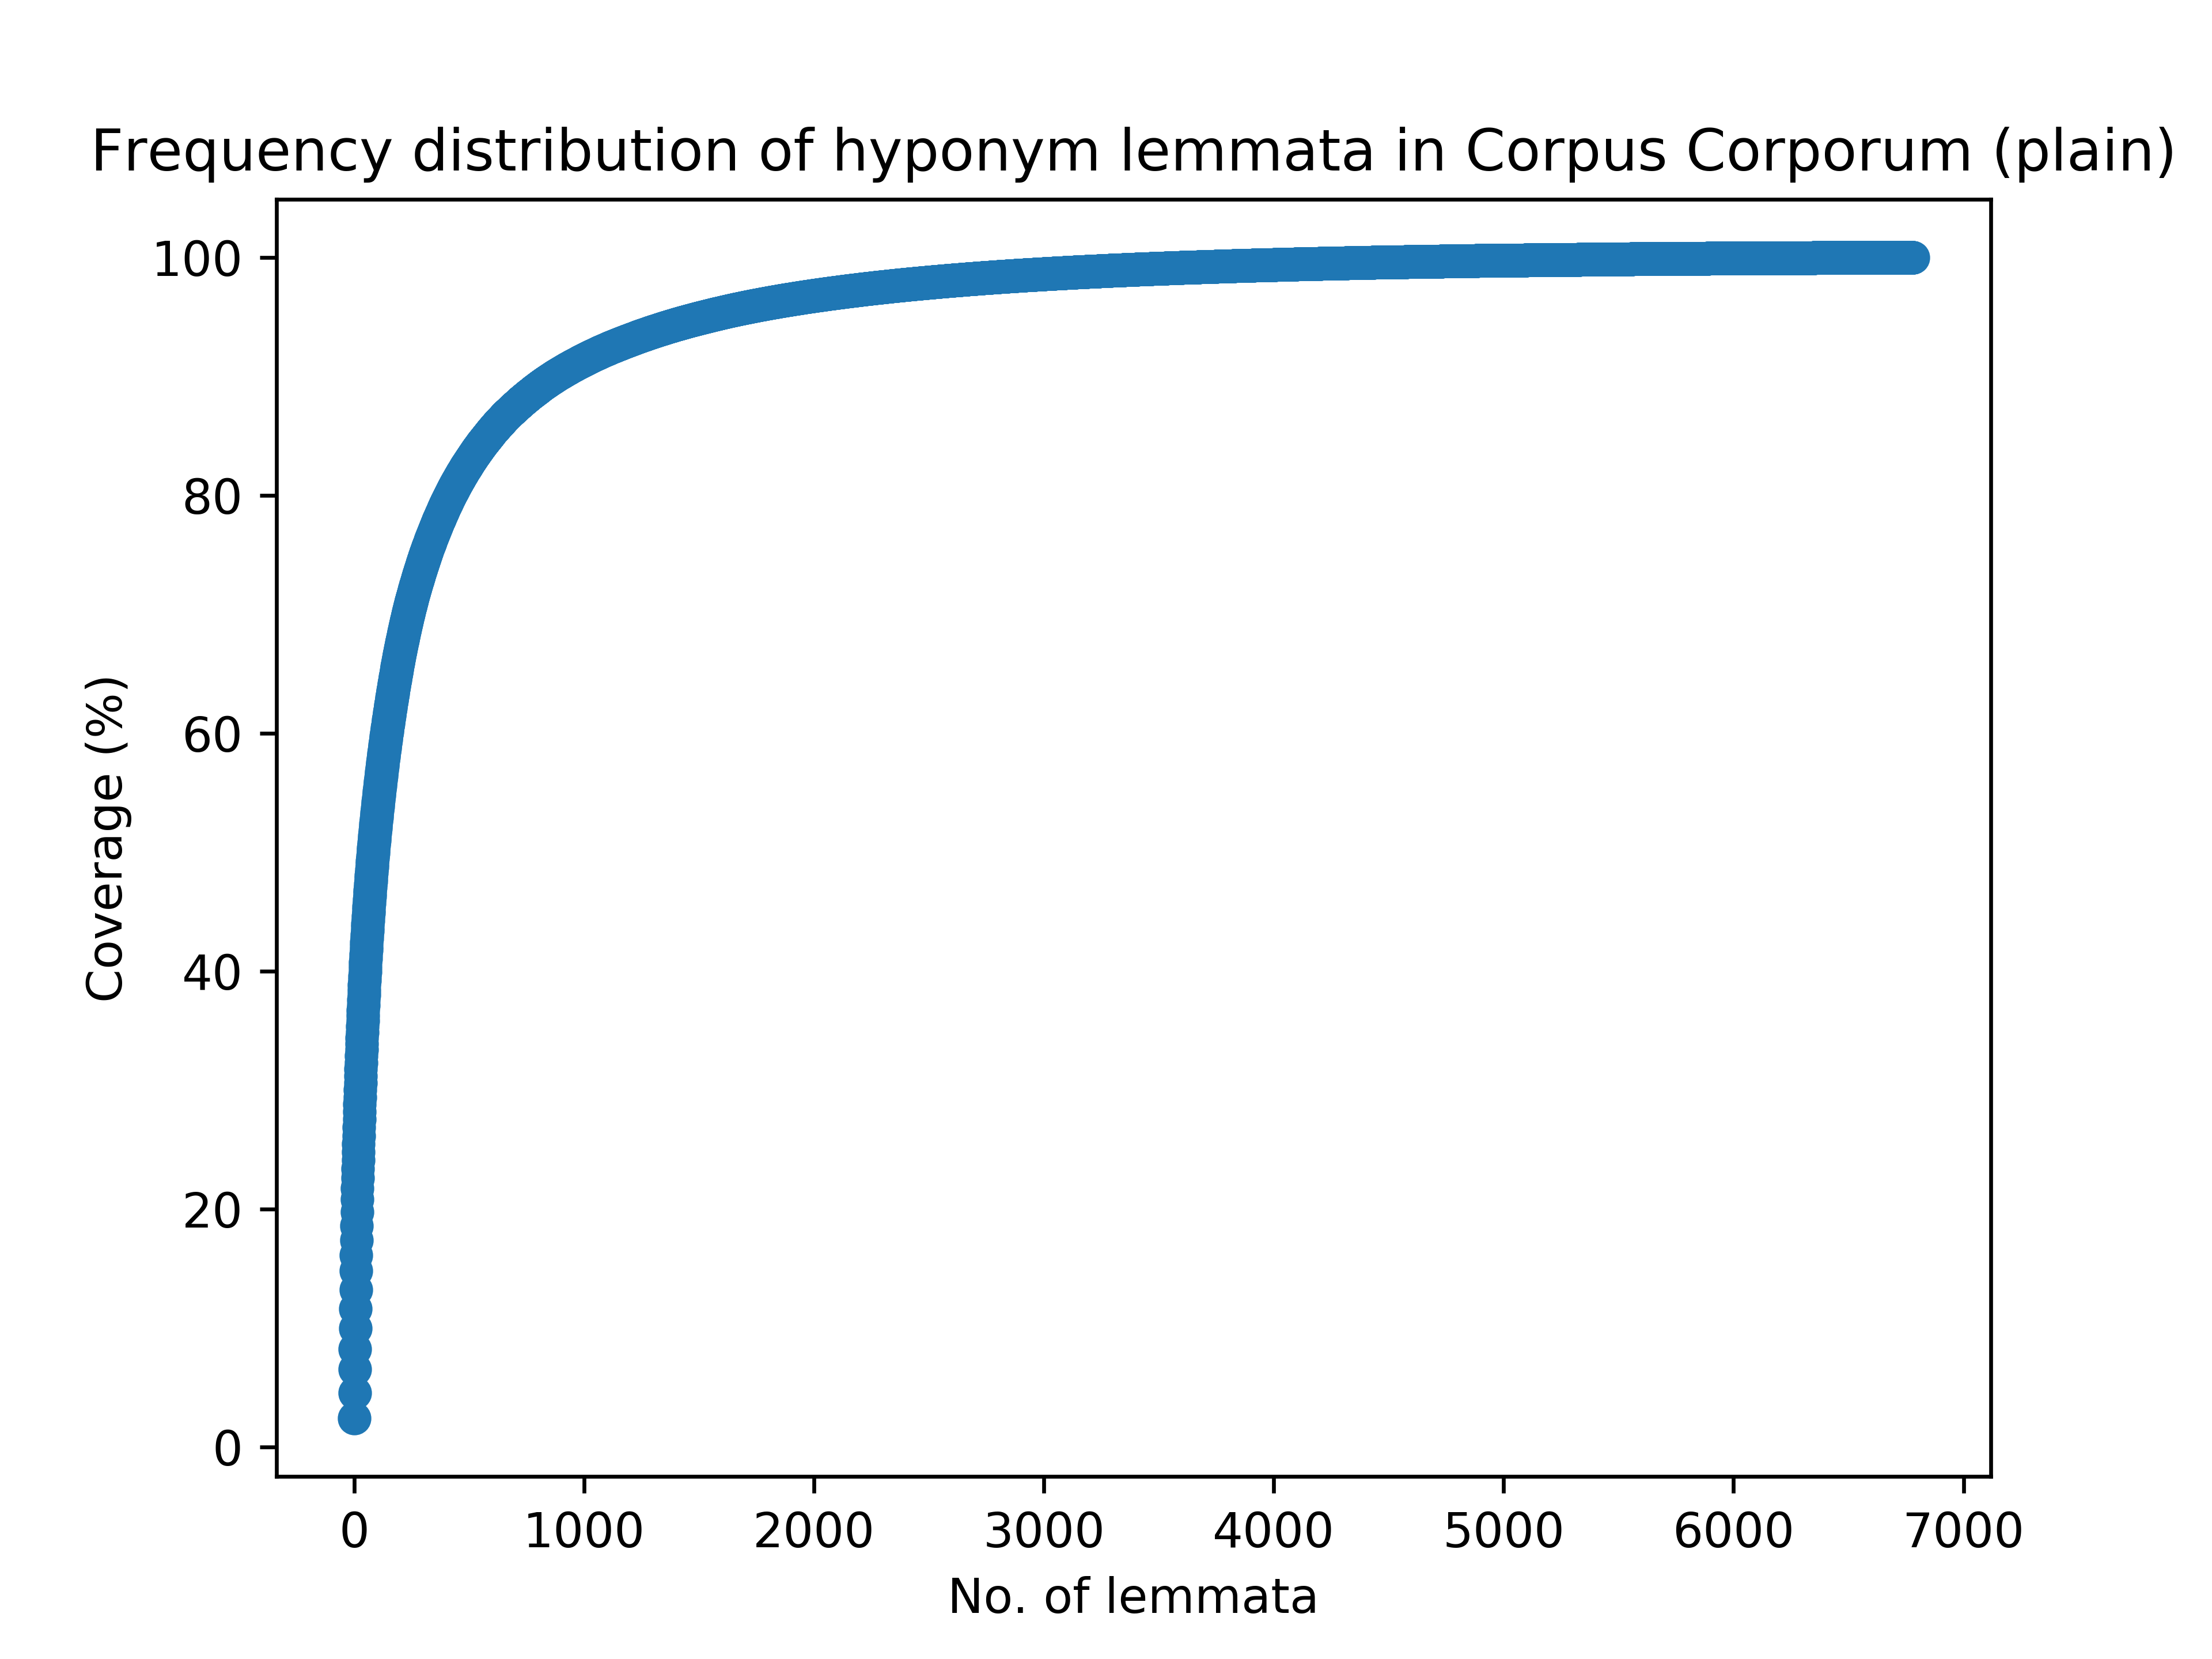
\includegraphics[width=\linewidth]{freq_dist_hyponyms_cc_plain}
\label{figure:frequencyDistributionHyponymsCCplain}
\end{figure}


\section{Appendix}

\subsection{Appendix A: Agile and Open Methodology}
\label{sec:appendixA}

This study will follow an approach which is borrowed from computer science, namely the agile methodology for software development:
\blockquote[{\cite[p.~32]{fowlerAgileManifesto2001}}]{[...] agile processes assume and encourage the alteration of requirements while the code is being written. As such, design cannot be a purely up-front activity to be completed before construction. Instead, design is a continuous activity that's performed throughout the project.}
Coding will be used to establish a proof of concept for this study by implementing the discussed models and testing them on real-world corpus data. Furthermore, the basic notion of incremental and iterative progress also applies to the way the models themselves are being created: The dissertation will see a range of approaches and considerations being applied for various purposes, which reflects my own thoughts about the detection of semantic relations growing from initial, very basic foundations (e.g. plain contingency tables) to more complex environments of semantic study. The application of agile methodology to linguistic research is motivated not just by the related coding activities, but also by the similarities between dissertations and software products: In this view, a dissertation can be seen as a product to be delivered to customers, i.e. the research community. The analogy is enhanced further by the overlapping quality factor of openness: Dissertations are necessarily products of open science in much the same way as open source software is the product of other communities sharing the desire for unrestricted public access to creative commons.
\blockquote[{\cite[p.~518]{garcia-penalvoOpenKnowledgeManagement2010}}]{We think that Open Knowledge comprises Open Software, Open Content, Open Science and Open Innovation. [...] Open Software owes its deepest roots to Open Access; Open Contents are related to open access to the educative, cultural or divulgative contents that are published under a non restrictive license that allows copy and distribution, but also the right to modify works. Open Science is devoted to the open access to scientific contents, while Open Innovation transfers the Open Access principles to the enterprise production world, which is actually indispensable for the enhancement of University-Enterprises relationships.}
To demonstrate the viability of this transfer, the dissertation is split into various modules, separating, e.g., the bibliography from the rest of the documents and employing cross-references to put it all together for presentational purposes. These modules are, to some extent, directly visible in the sense of multiple source files that may be compiled to form a more complex document. Also, they are all publicly accessible at \href{https://github.com/konstantinschulz/asrael} and subject to version control, thus enabling readers to trace the resulting thoughts back to their very roots. Eventually, the reason to make all these considerations explicit is not so much to suggest a high quality of the work process, but rather to emphasize their possibly tremendous influence on the results and how they are gathered.


\printbibliography[heading=bibintoc]

\end{document}
























